% -----------------------------------------------
% Vlastní text práce (kapitoly práce)
% -----------------------------------------------

% -----------------------------------------------
\chapter{Gamma rays detection}
% -----------------------------------------------


% -----------------------------------------------
\section{Properties and parameters of detectors}
% -----------------------------------------------
The main parameters of interest for Mössbauer spectroscopy are detection efficiency and energy resolution at low gamma energies. Nowadays, three main types of detectors are used in nuclear physics - gas, scintillation and semiconductor. The Mössbauer spectrometer setups in the laboratories of the Department of Experimental Physics (DEP) of Palacky University are usually based on gas or scintillation detectors.
%The main parameters which are crucial for purposes of Mössbauer spectroscopy are detection efficiency and energy resolution at low gamma energies. Nowadays three main types of detectors are employed on the field of nuclear physics - gas, scintillation and semiconductor. The Mössbauer spectrometer setups in laboratories of Department of Experimental Physics (DEP) of Palacky University are usually based on gas or scintillation detectors.


\subsection{Gas proportional detectors}
The gas detectors are usually tubes with two electrodes filled with a special gas mixture. A gas tube LND45479, which  will be used for experiments in the following chapters, is shown in the figure \ref{gas}. The incoming particle ionises the gas, producing free ions and electrons. Gas detectors are operated in the proportional regime, which is characterised by proportional amplification of the charge carriers. The advantage of gas detectors is that they offer good energy resolution, but on the other hand their detection efficiency is low, mainly due to the fact that the gas density is low. Count rates are also affected by the long duration of the ionisation effect. They require high voltages (typically over 1000 V) to operate and, in the case of flow counters they also require pressure cylinders.
%The gas detectors are usually tubes with two electrodes filled with a special gas mixture. A gas tube we use for experiments in following chapters can be seen in the figure \ref{gas}. The incoming particle ionizes the gas, creating free ions and electrons. Gas detectors are operated in proportional regime, which is characterized by proportional amplification of charge carriers. The advantage of gaseous detectors is that they offer good energy resolution, but on the other hand their detection efficiency is low mainly due to the fact, that the gas density is small. Count rates are also affected by the long duration of the ionization effect. For operation, they require high voltages (usually over 1000 V) and in case of flow counters they also require pressure cylinders. 

\begin{figure}[H]
 \centering
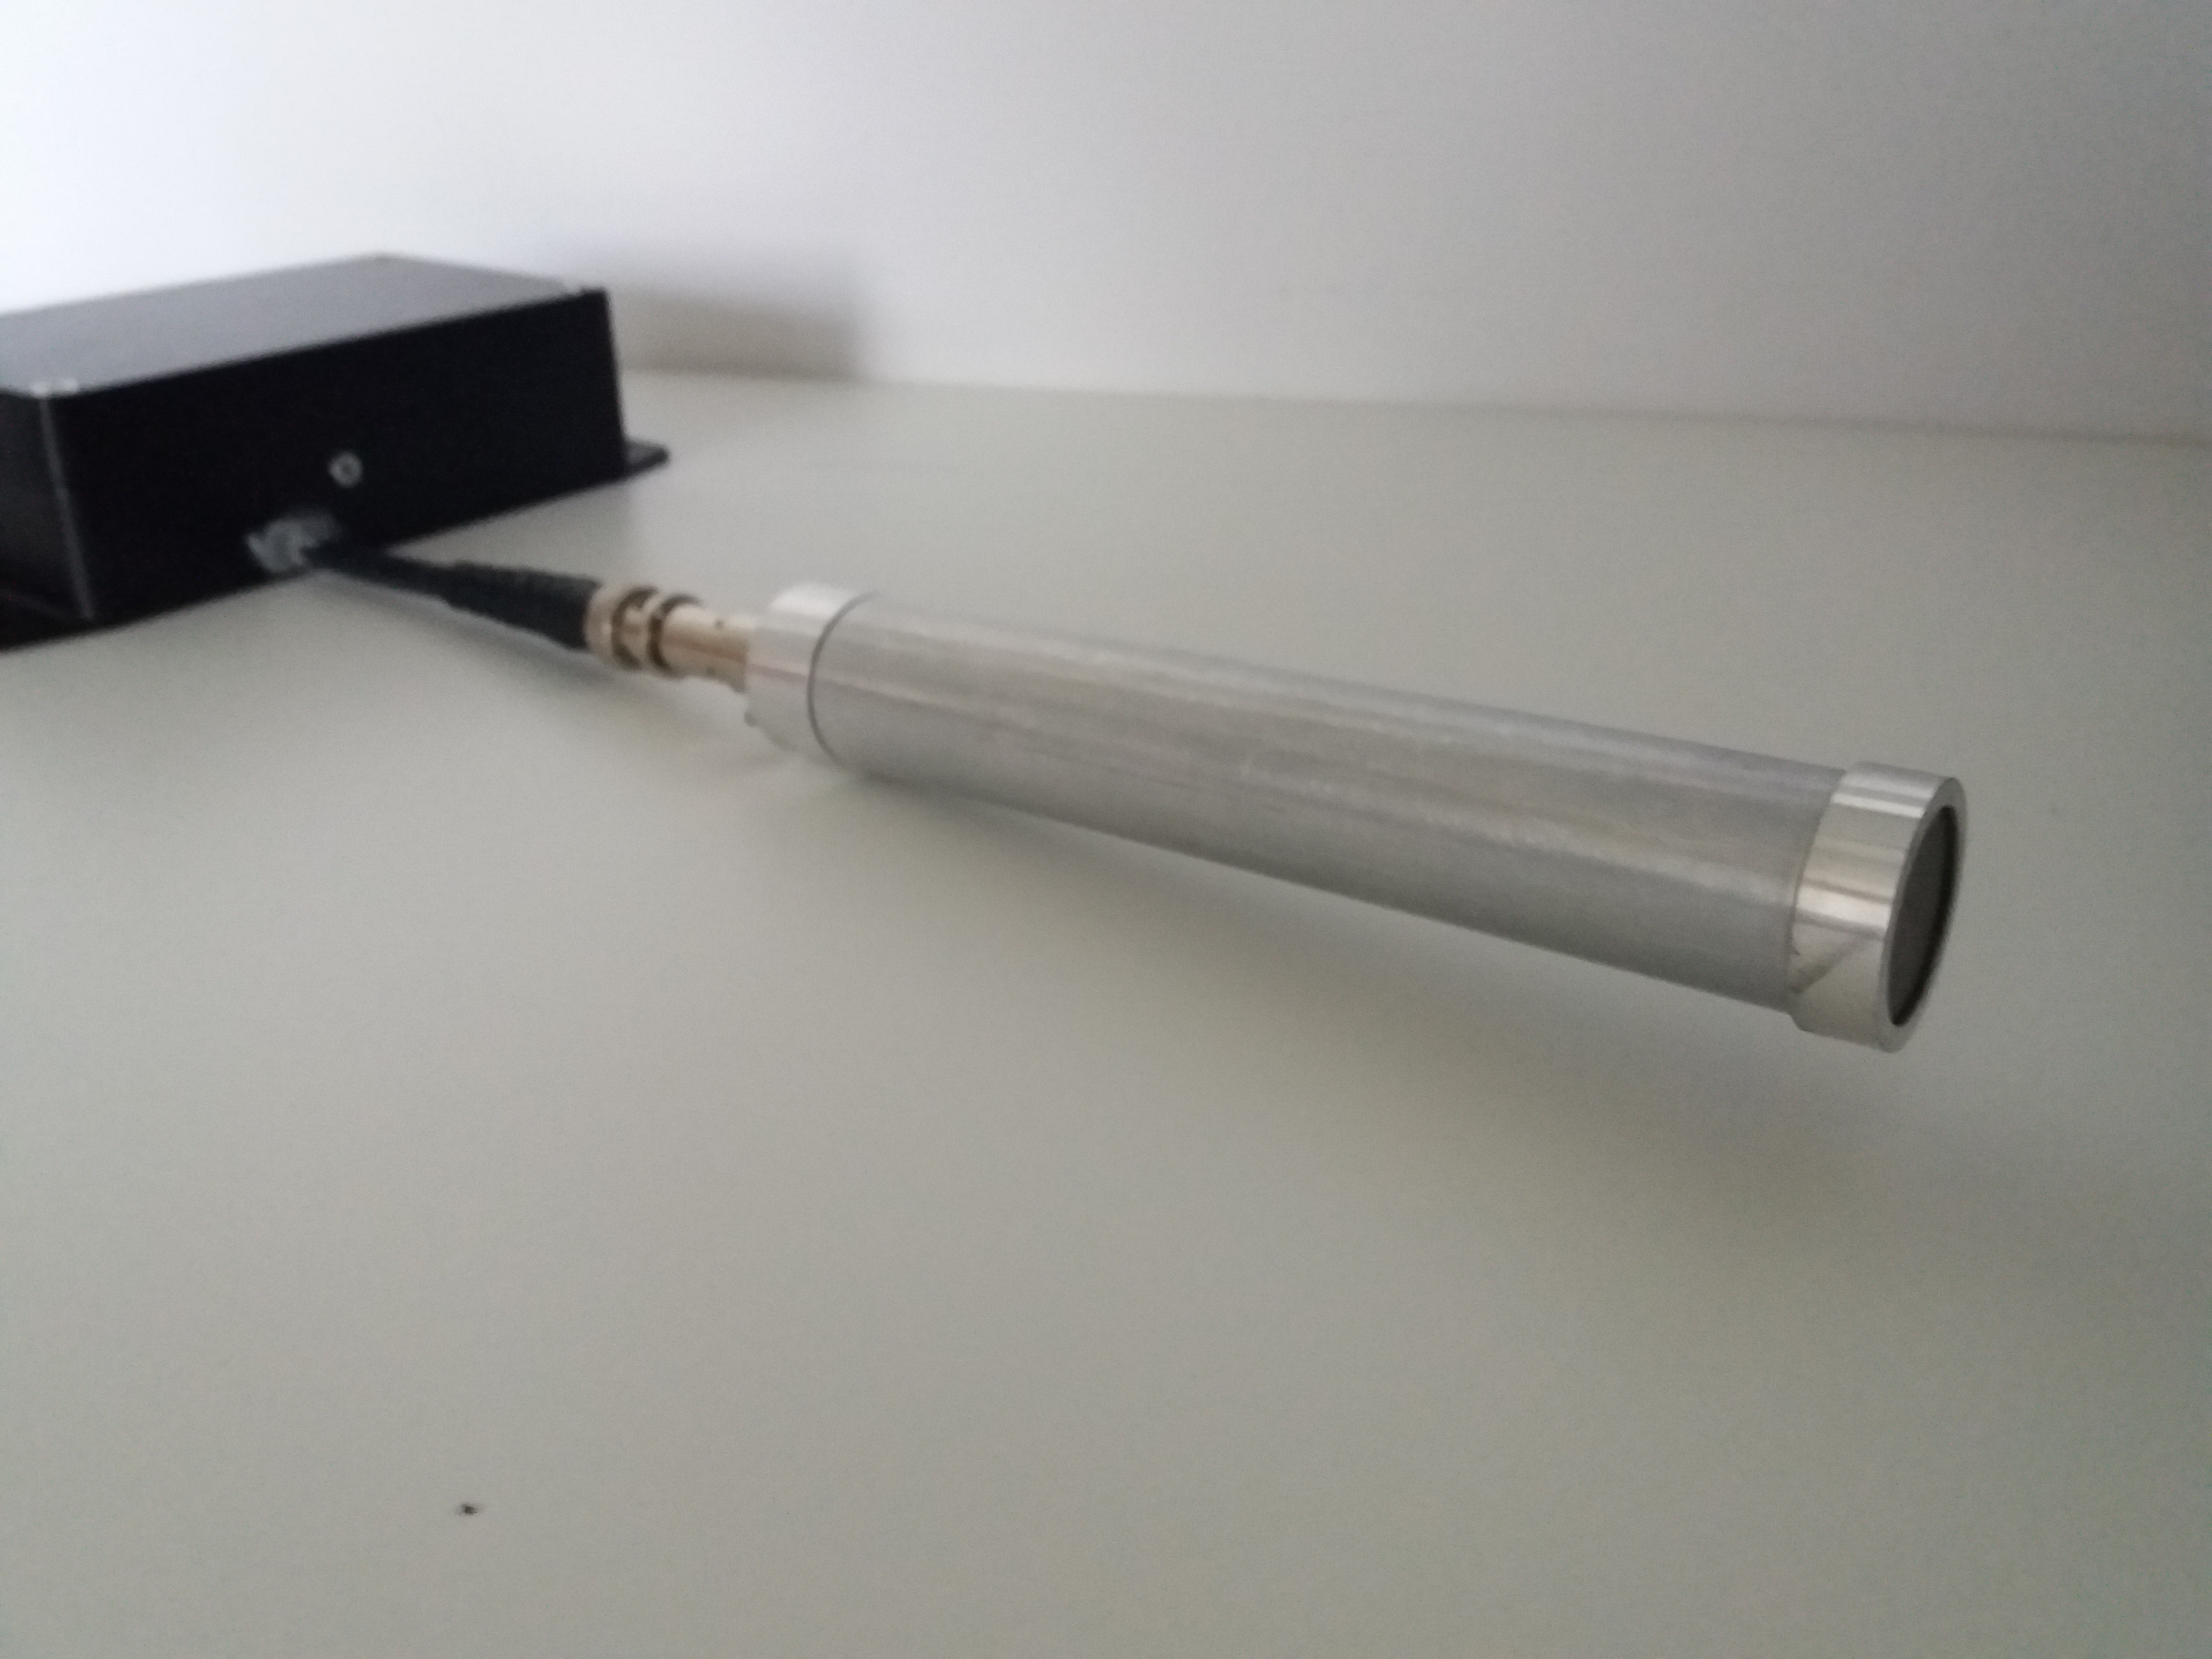
\includegraphics[scale=0.1, angle = 0]{./pictures/GasTube.jpg}
 \caption{Gas proportional detector LND45479.}
 \label{gas}
 
\end{figure}


\subsection{Scintillation detectors}
A scintillation detector is usually a scintillation crystal coupled to a photomultiplier tube (PMT). A scintillation detector (PMT R6095 with YAP(Ce) crystal) used later in this thesis can be seen in the figure \ref{scintillator}. The first conversion of photon energy takes place inside the scintillation crystal, where the incoming particle produces a number of photons linearly dependent on its energy. These photons are captured by the photocathode of the PMT, where they are converted into electrons and then amplified on the dynodes of the PMT. This amplification requires high voltages (from $500$V). The gain inside the PMT can be around $10^6$.
\par
The detection efficiency is very high and, due to the short excitation time, they can be used at high count rates. However, their energy resolution is much worse than in the case of gas detectors and semiconductors. The resulting gamma spectra tend to have distorted broad peaks, which negatively affects Mössbauer spectroscopy - reduces SNR. 
%A scintillation detector is usually meant a scintillation crystal coupled with a photomultiplier tube (PMT). A scintillation detector (PMT R6095 with YAP(Ce) crystal) used later in this thesis can be seen in the figure \ref{scintillator}. The first conversion of the photon energy happens inside the scintillation crystal where the incoming particle generates number of photons linearly dependent on its energy. These photons are captured by PMT's photocathode, where they are converted into electrons, and then multiplied on PMT's dynodes. This amplification requires high voltages (starting from $500$ V). The amplification inside PMT can be around $10^6$.
%\par
%The detection efficiency is very high and due to the short duration of excitation process, they can be used at high count rates. However, their energy resolution is much worse than in case of gas detectors and semiconductors. The gamma spectra obtained this way usually have distorted wide peaks, which negatively affects Mössbauer spectroscopy - decreases SNR. 

%Also the employment of PMTs inside the magnetic fields is very problematic and requires a difficult instrumentation.

\begin{figure}[H]
 \centering
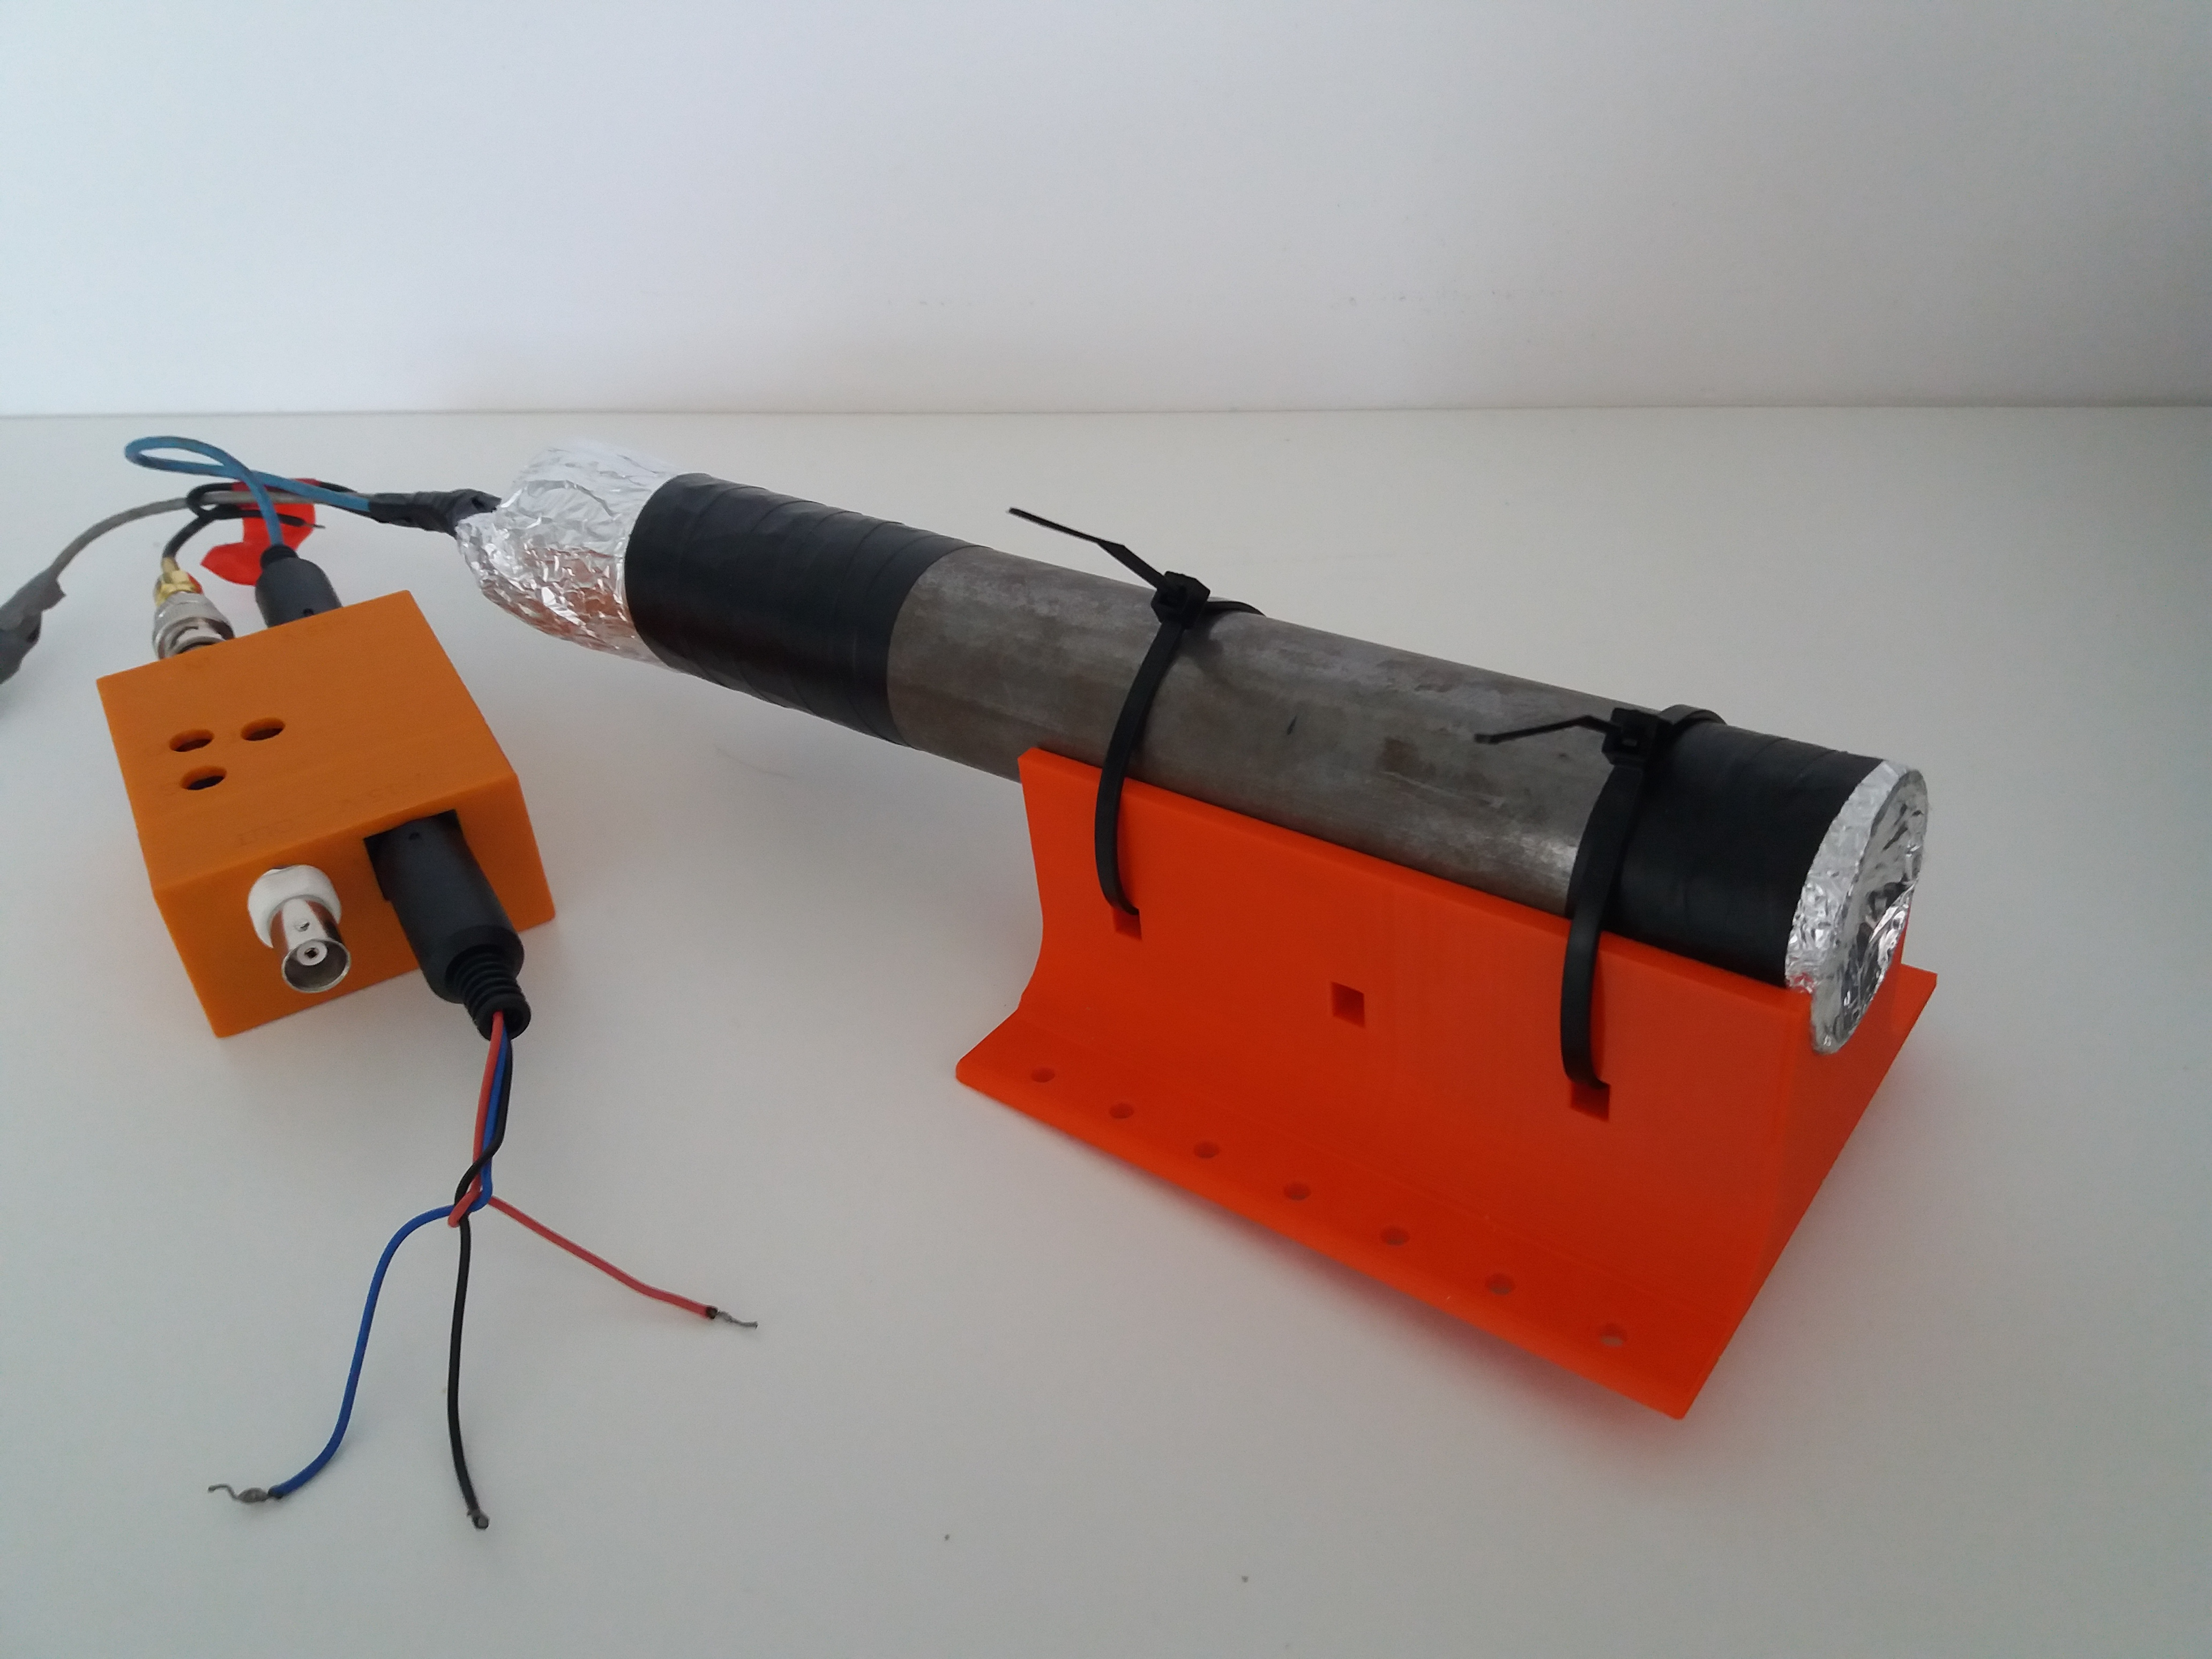
\includegraphics[scale=0.1, angle = 0]{./pictures/Scintillator.jpg}
 \caption{Scintillation detector with amplifier. PMT (R6095) and scintillation crystal (YAP(Ce)) are inside the metal tube.}
 \label{scintillator}
 
\end{figure}


\subsection{Detectors based on semiconductors}
Semiconductors offer the best energy resolution - the energy required to produce a charge carrier is usually very small (in the order of eV). Detection efficiency depends on the energy of the gamma photon and the thickness of the detector. The efficiency can be very high - for example, some Si PIN diodes have efficiencies close to 100 $\%$ up to 10 keV \cite{SiCdTe}.
\par
However, semiconductors are usually more expensive than the other types of detectors. They can be used as direct radiation detectors, or they can be coupled with a scintillator crystal.
\par
One problem with semiconductor detectors is that there is no internal amplification, so the signals coming out of the detectors have to be heavily amplified by electronics.
On the other hand, they are small and compact. They also don't require high voltage sources or heavy pressure cylinders to operate. These facts are crucial when it comes to building more compact Mössbauer spectrometers - for example, MIMOS II \cite{https://doi.org/10.1029/2003JE002138}, based on 4 Si PIN diodes, was part of the two rovers Spirit and Opportunity on their mission to Mars.
%The semiconductors offer the best energy resolution - the energy required to create a charge carrier is usually very small (in order of eVs). The detection efficiency depends on gamma photon's energy and detector thickness. The efficency can be very high - for example some Si PIN diodes have their efficency near 100 $\%$ up to 10 keV \cite{SiCdTe}.
%\par
%However, semiconductors are usually more expensive than the other types of detectors. They can be used as direct radiation detectors or there is also a possibility to couple them with a scintillator crystal.
%\par
%One problem with semiconductor detector is that there is no internal amplification, so the signals coming out of the detectors have to be strongly amplified by electronics.
%On the other hand, they are small and compact. They also don't require high voltage sources or heavy pressure cylinders to operate. These facts are crucial if it comes to making more compact Mössbauer spectrometers - for example MIMOS II \cite{https://doi.org/10.1029/2003JE002138} based on 4 Si PIN diodes was a part of two rowers Spirit and Opportunity on their mission on Mars. 




% %%%%%%%%%%%%%%%%%%%%%%%% End of file %%%%%%%%%%%%%%%%%%%%%%%%